%************************************************
\chapter{First-order Reflective Thinking}
\label{chapter:first_order_refective_thinking}
%************************************************

\section{Static Spatial Arrangements}

Spatial arrangements of static symbols are created by the reflective
thinking layers.  Static symbols are not contained within the physical
layer, but these symbols are used to represent transitions from the
past to the future, which are in turn used to create relationships
between causes and effects that are used for planning.  Thinking
activities use these Spatial arrangements of symbols to think about
the given activities of the physical layer as well as planning in the
first-order reflective layer.

\section{Simultaneities}

{\mbox{\autoref{figure:example_simultaneity}}} shows an example
simultaneity.
\begin{figure}
\center
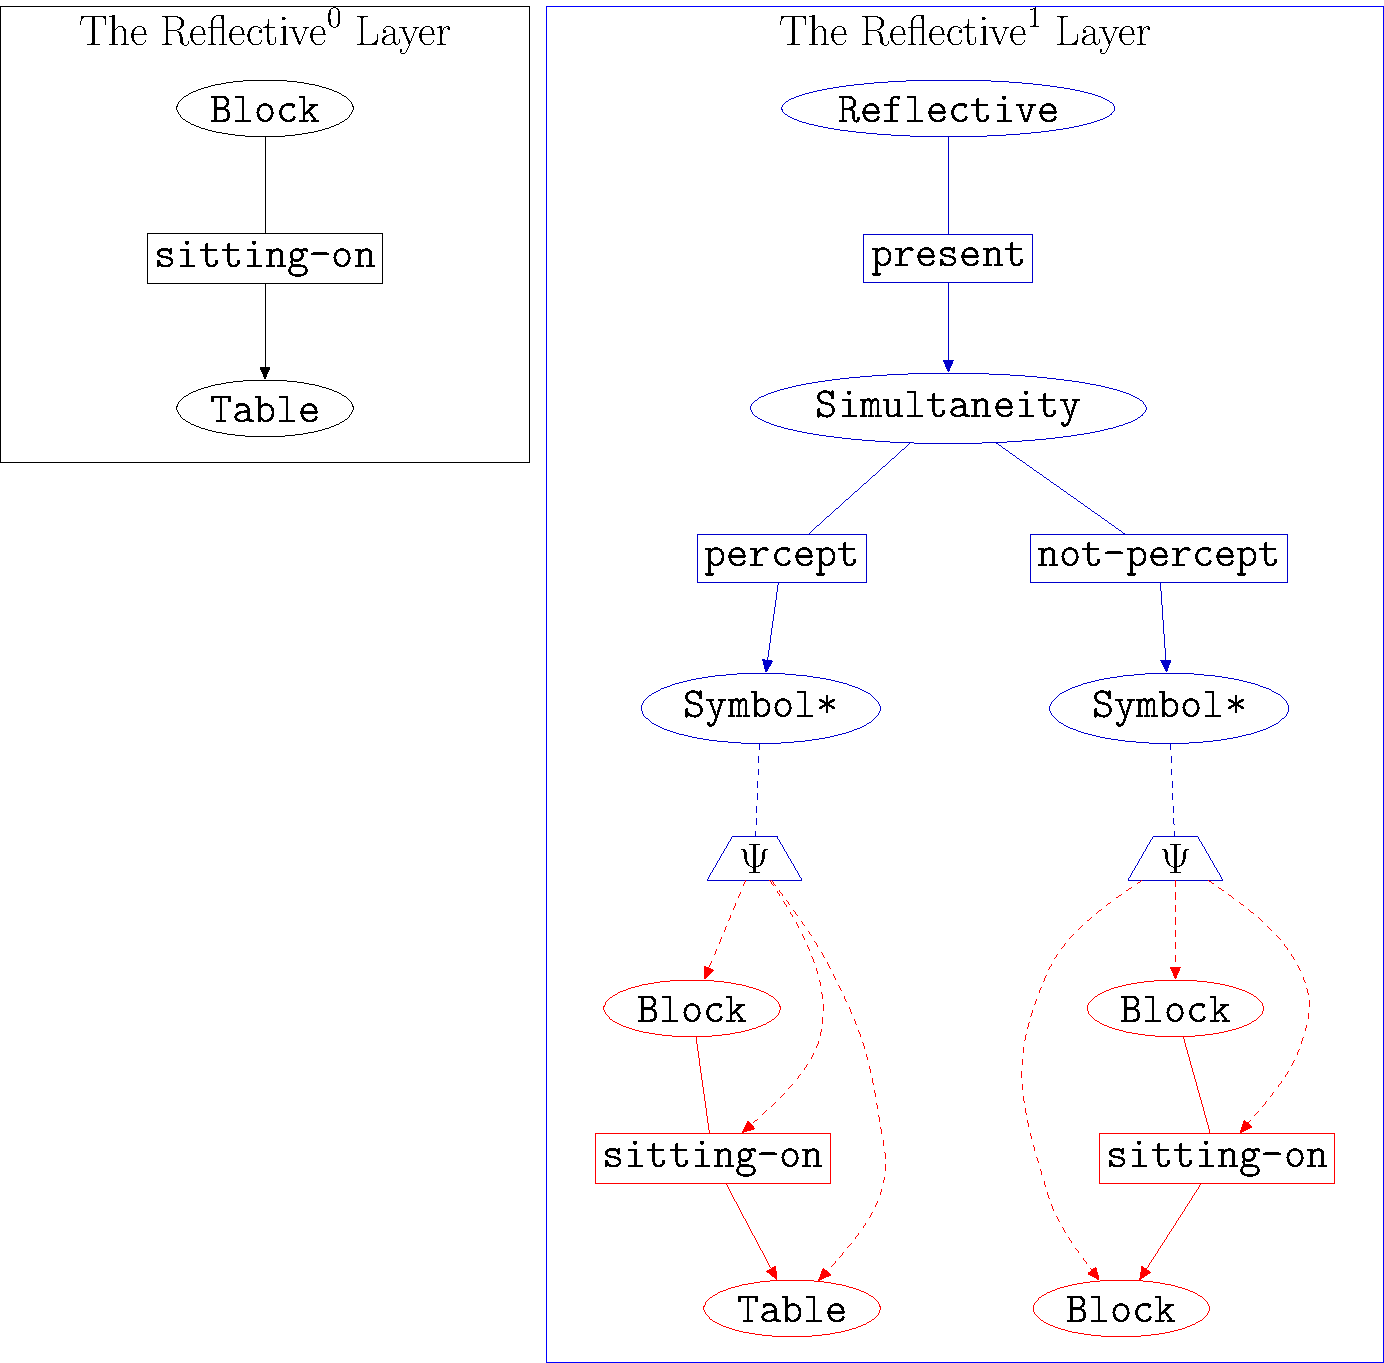
\includegraphics[width=10cm]{gfx/example_simultaneity}
\caption[Example simultaneity of positive and negative symbolic
  perceptions.]{Example simultaneity, $\text{\tt{simult}}_1^*$, of
  positive and negative symbolic perceptions, where the symbolic
  reference to physical activity, $x_1^*$, is perceived, while $x_2^*$
  is not.}
\label{figure:example_simultaneity}
\end{figure}

\section{Transitions}

As {\mbox{\autoref{equation:define_symbol_referent_graph}}} states,
each reflective thinking layer can create symbolic references to
dynamic activities in the layers below as well as any other symbolic
activities in or below the symbolization activity.  Simultaneities and
transitions are the basis for representing concurrent and sequential
event knowledge.  It is a type of static Spatial arrangement between
static symbolic references.  Simultaneities and transitions can be
arranged into sequences back in time, forward in time, as well as
organizing time into binary trees for efficient recall.
\begin{figure}
\center
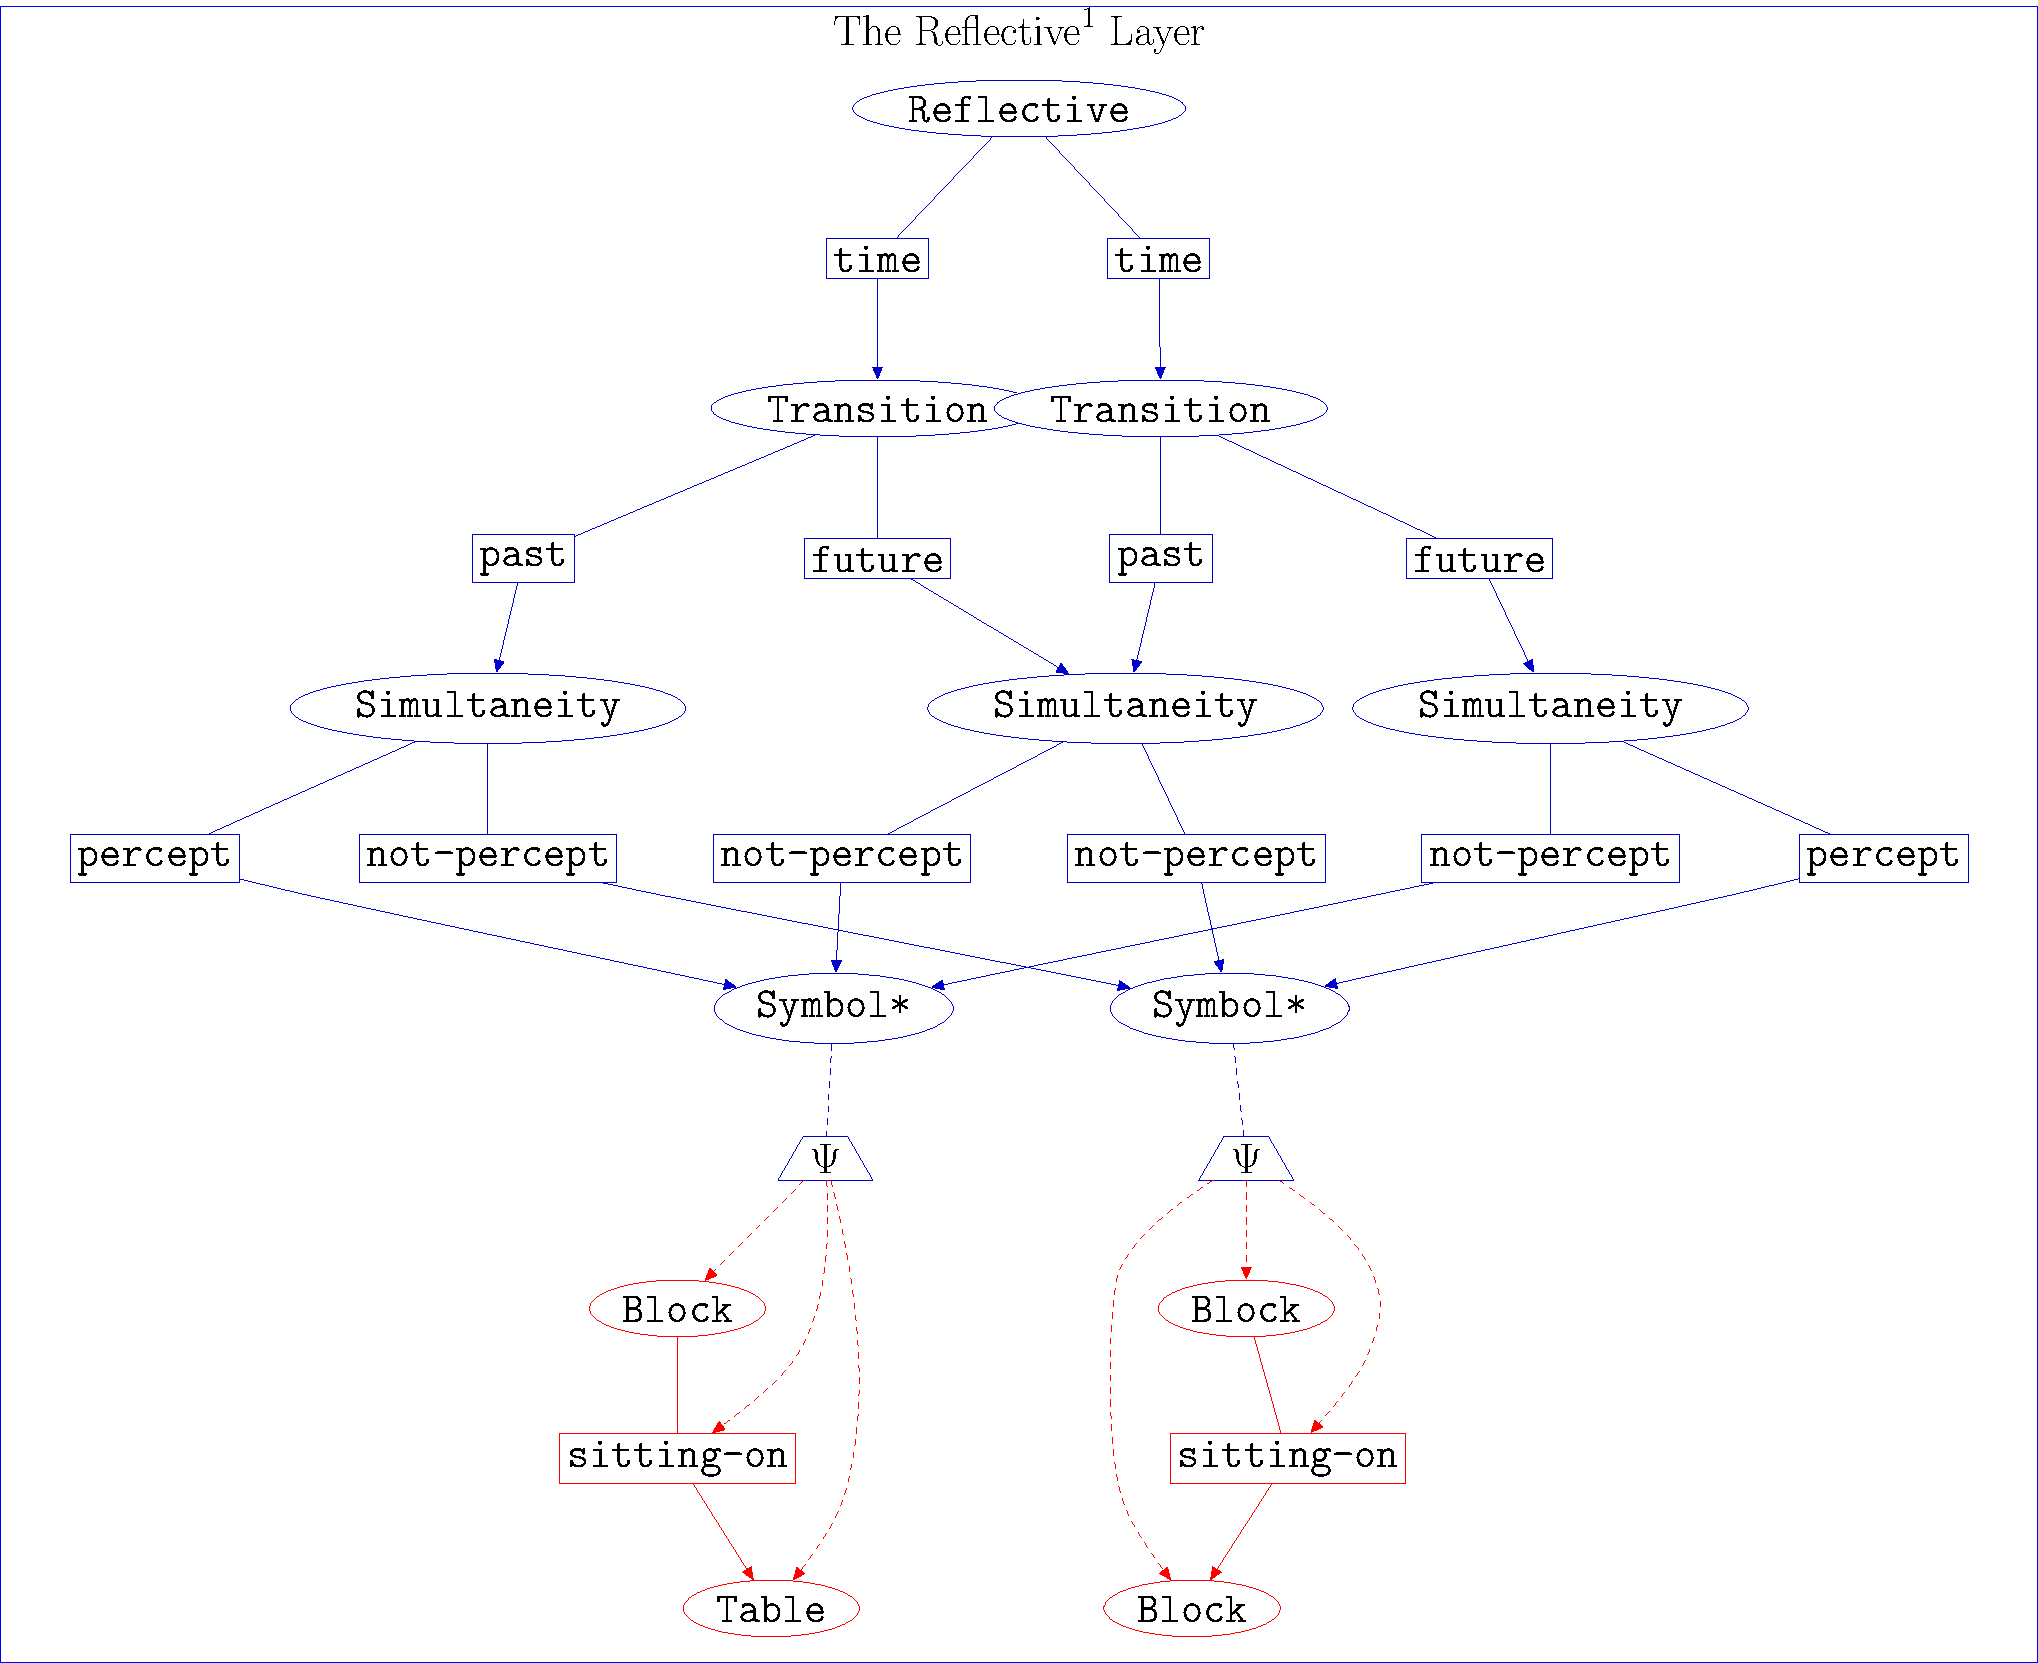
\includegraphics[width=12cm]{gfx/example_transition}
\caption[An example of a transition between simultaneities.]{An
  example of a transition between simultaneities,
  $\text{\tt{simult}}_1^*$ and $\text{\tt{simult}}_2^*$, which
  represent the transition between perceiving the first-order static
  symbolic reference, $x_1^*$, and then subsequently, $x_2^*$.}
\label{figure:example_transition}
\end{figure}

\section{Transframes}

While transitions represent a temporal relationship between two
simultaneities, a \emph{transframe} is an abstracted object that only
represents the differences between two of these simultaneities.  For
example, two states could both contain a lot of perceptual
information, but the transframe between them might be a very small set
of differences.  The changes of a transframe are kept track of as
additions and removals of various simultaneities that are contained
within the past or the future simultaneities of a transition
relationship.  {\mbox{\autoref{figure:example_transframe}}} shows two
examples of transframes that could be abstracted from the transition
in {\mbox{\autoref{figure:example_transition}}}.
\begin{figure}
\center
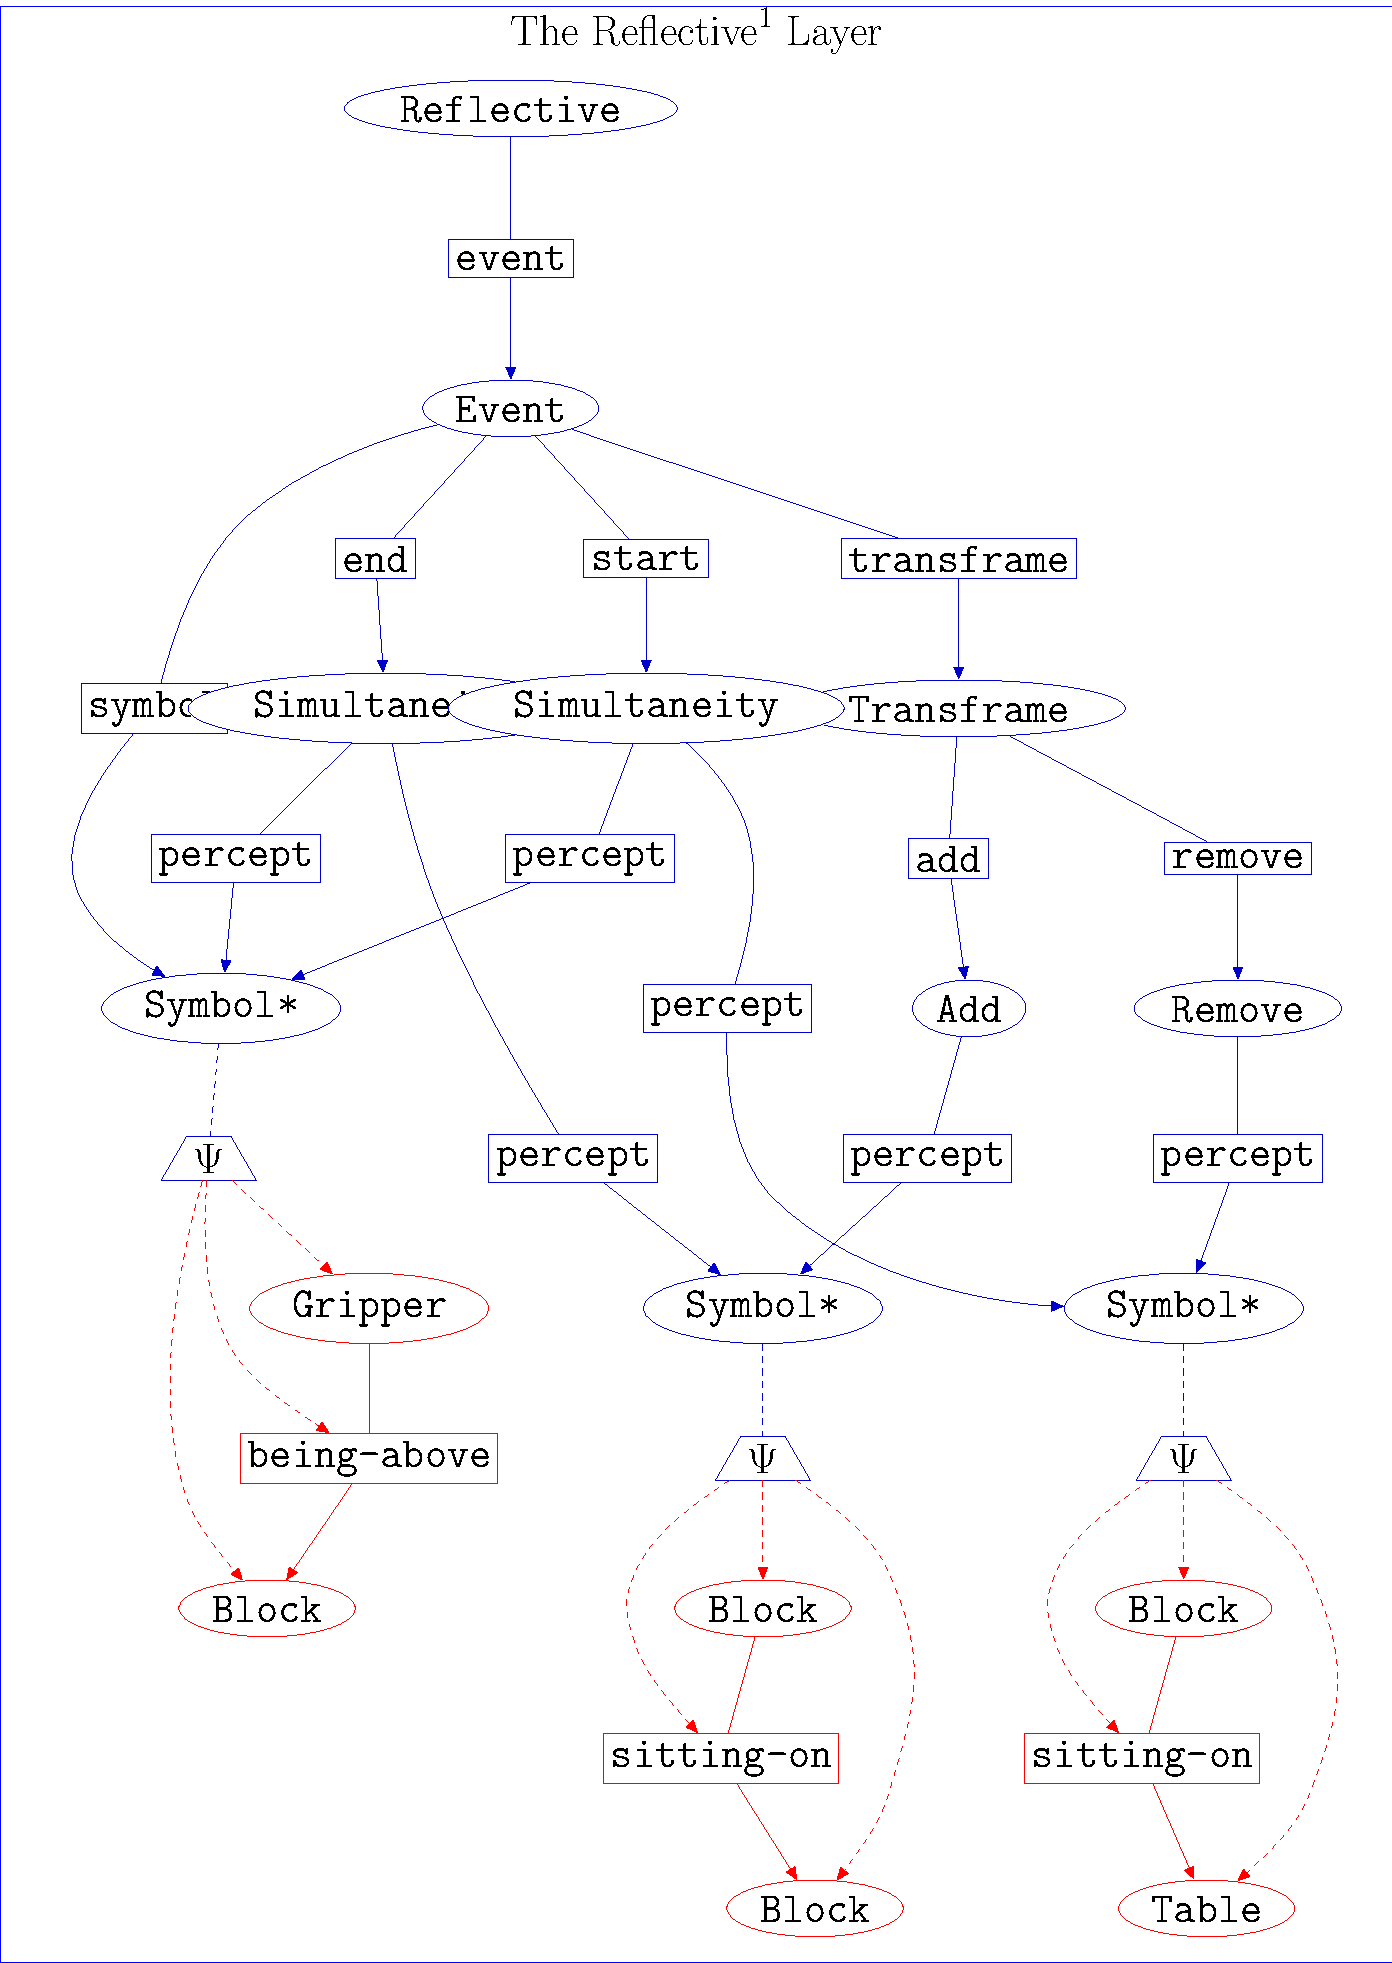
\includegraphics[width=12cm]{gfx/example_transframe}
\caption[Two examples of transframes.]{Two examples of transframes
  that can be abstracted from the transition in
  {\mbox{\autoref{figure:example_transition}}}.}
\label{figure:example_transframe}
\end{figure}

\section{Causal Knowledge}

{\mbox{\autoref{figure:example_causal_knowledge}}} shows an example of
causal knowledge.
\begin{figure}
\center
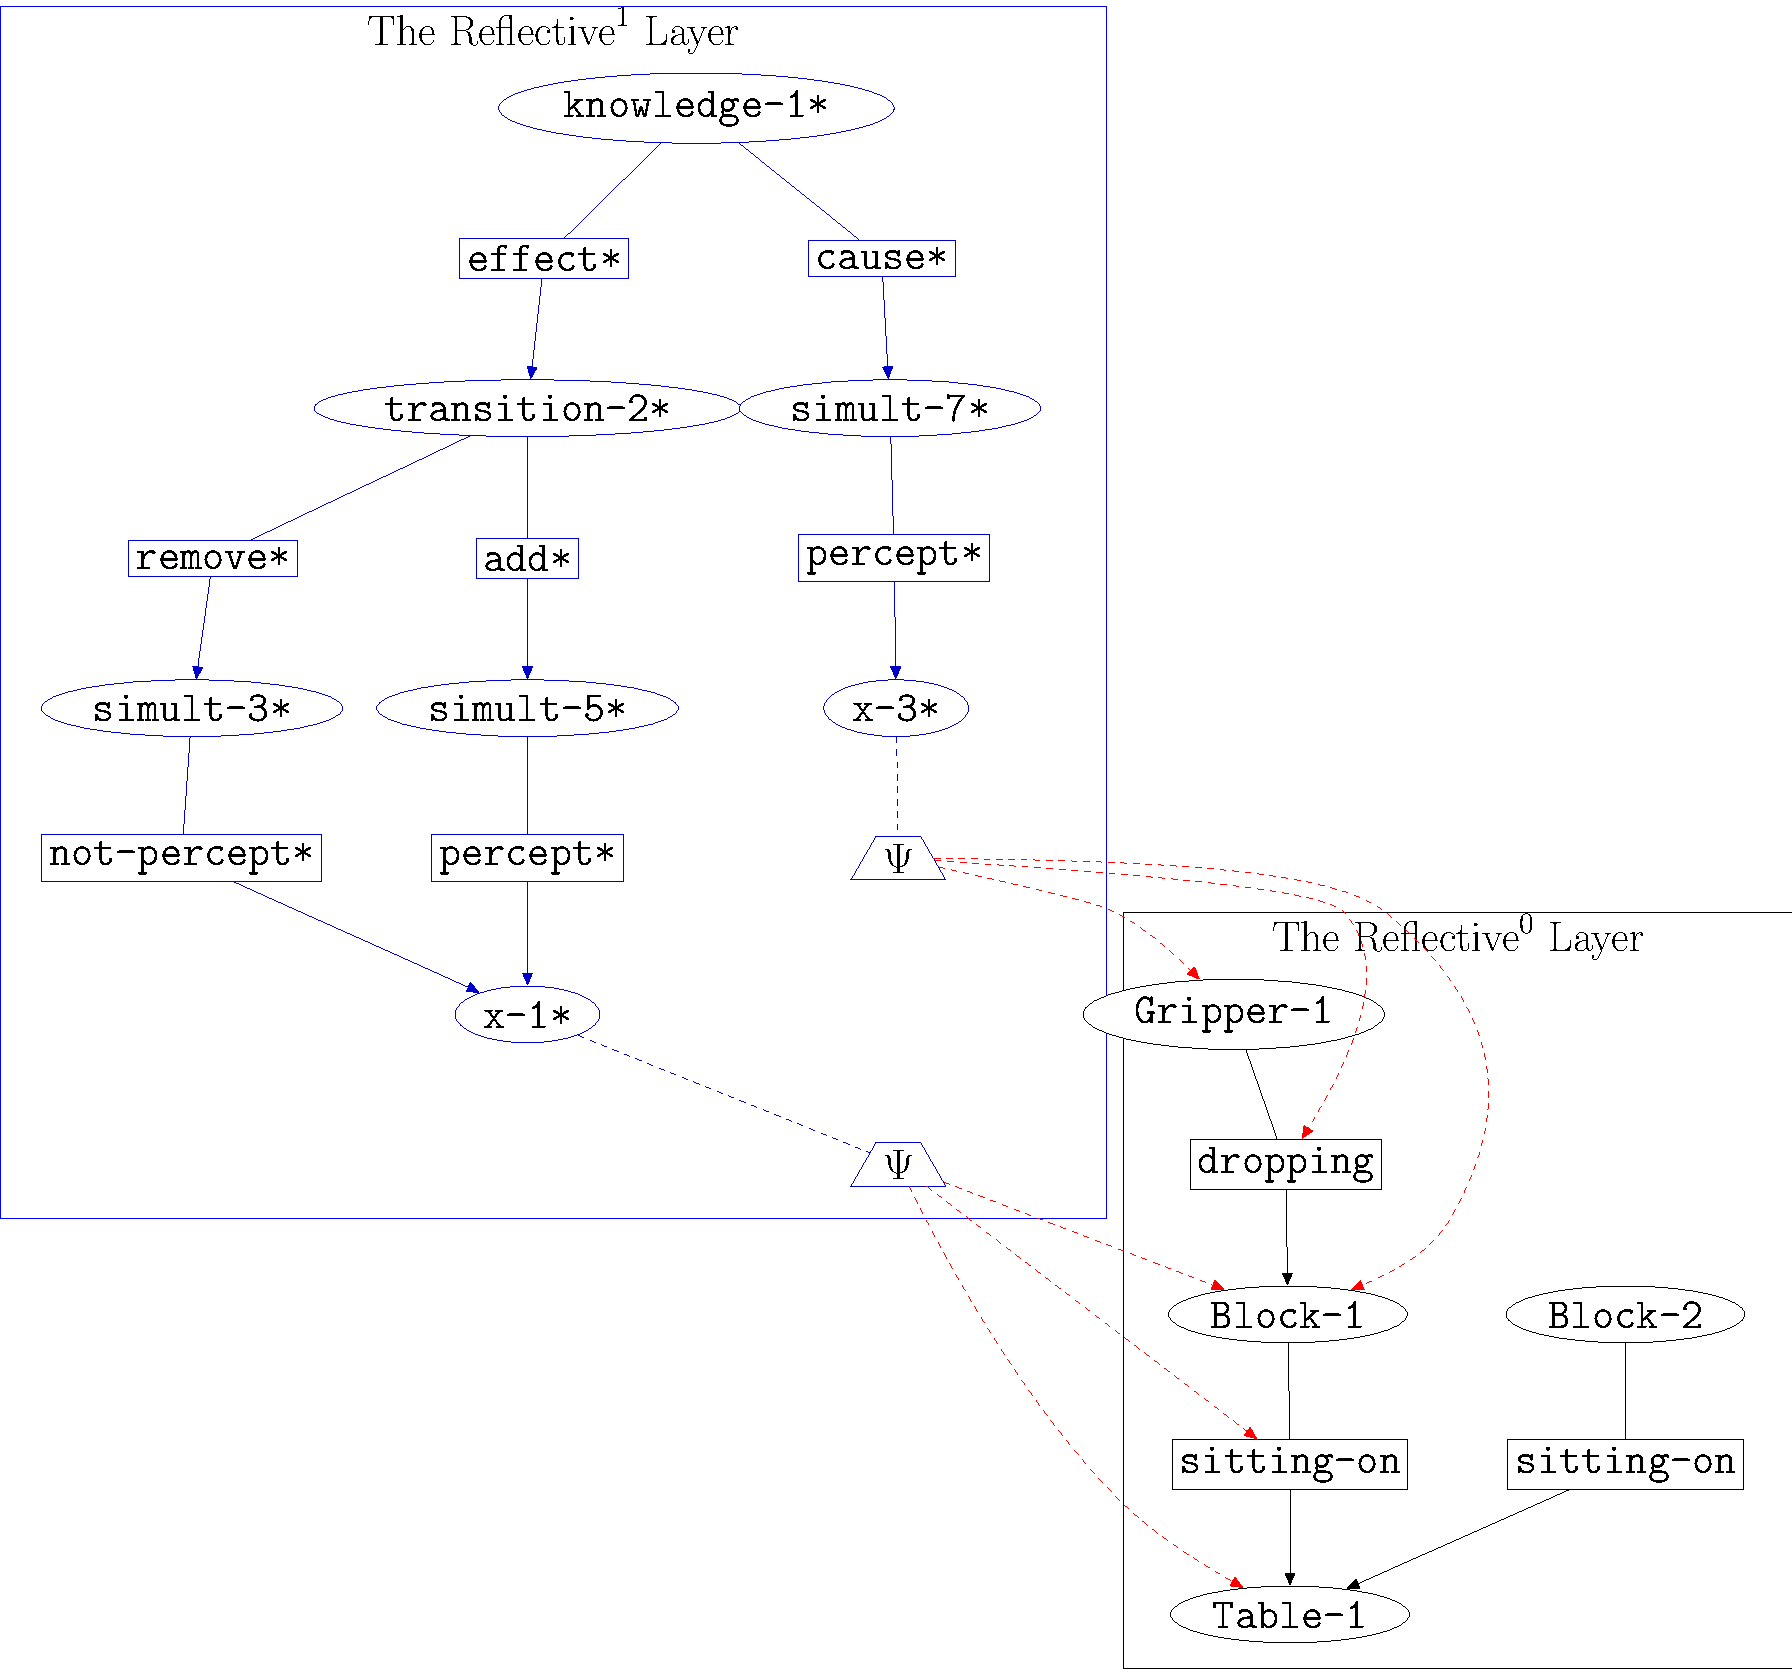
\includegraphics[width=12cm]{gfx/example_causal_knowledge}
\caption[An example of a causal hypothesis.]{An example of causal
  knowledge, $\text{\tt{knowledge}}_1^*$, where the simultaneity,
  $\text{\tt{simult}}_7^*$, is known to be the cause of the
  transframe, $\text{\tt{transition}}_2^*$.}
\label{figure:example_causal_knowledge}
\end{figure}

\section{Representing Causal Hypotheses}

{\mbox{\autoref{figure:example_causal_hypothesis}}} shows an example
of a causal hypothesis, $h_1^*$, where the simultaneity,
$\text{\tt{simult}}_7^*$, is hypothesized to be the cause of the
transframe, $\text{\tt{transframe}}_2^*$.  In other words, the gripper
dropping the block causes the block to be sitting on the table.
\begin{figure}
\center
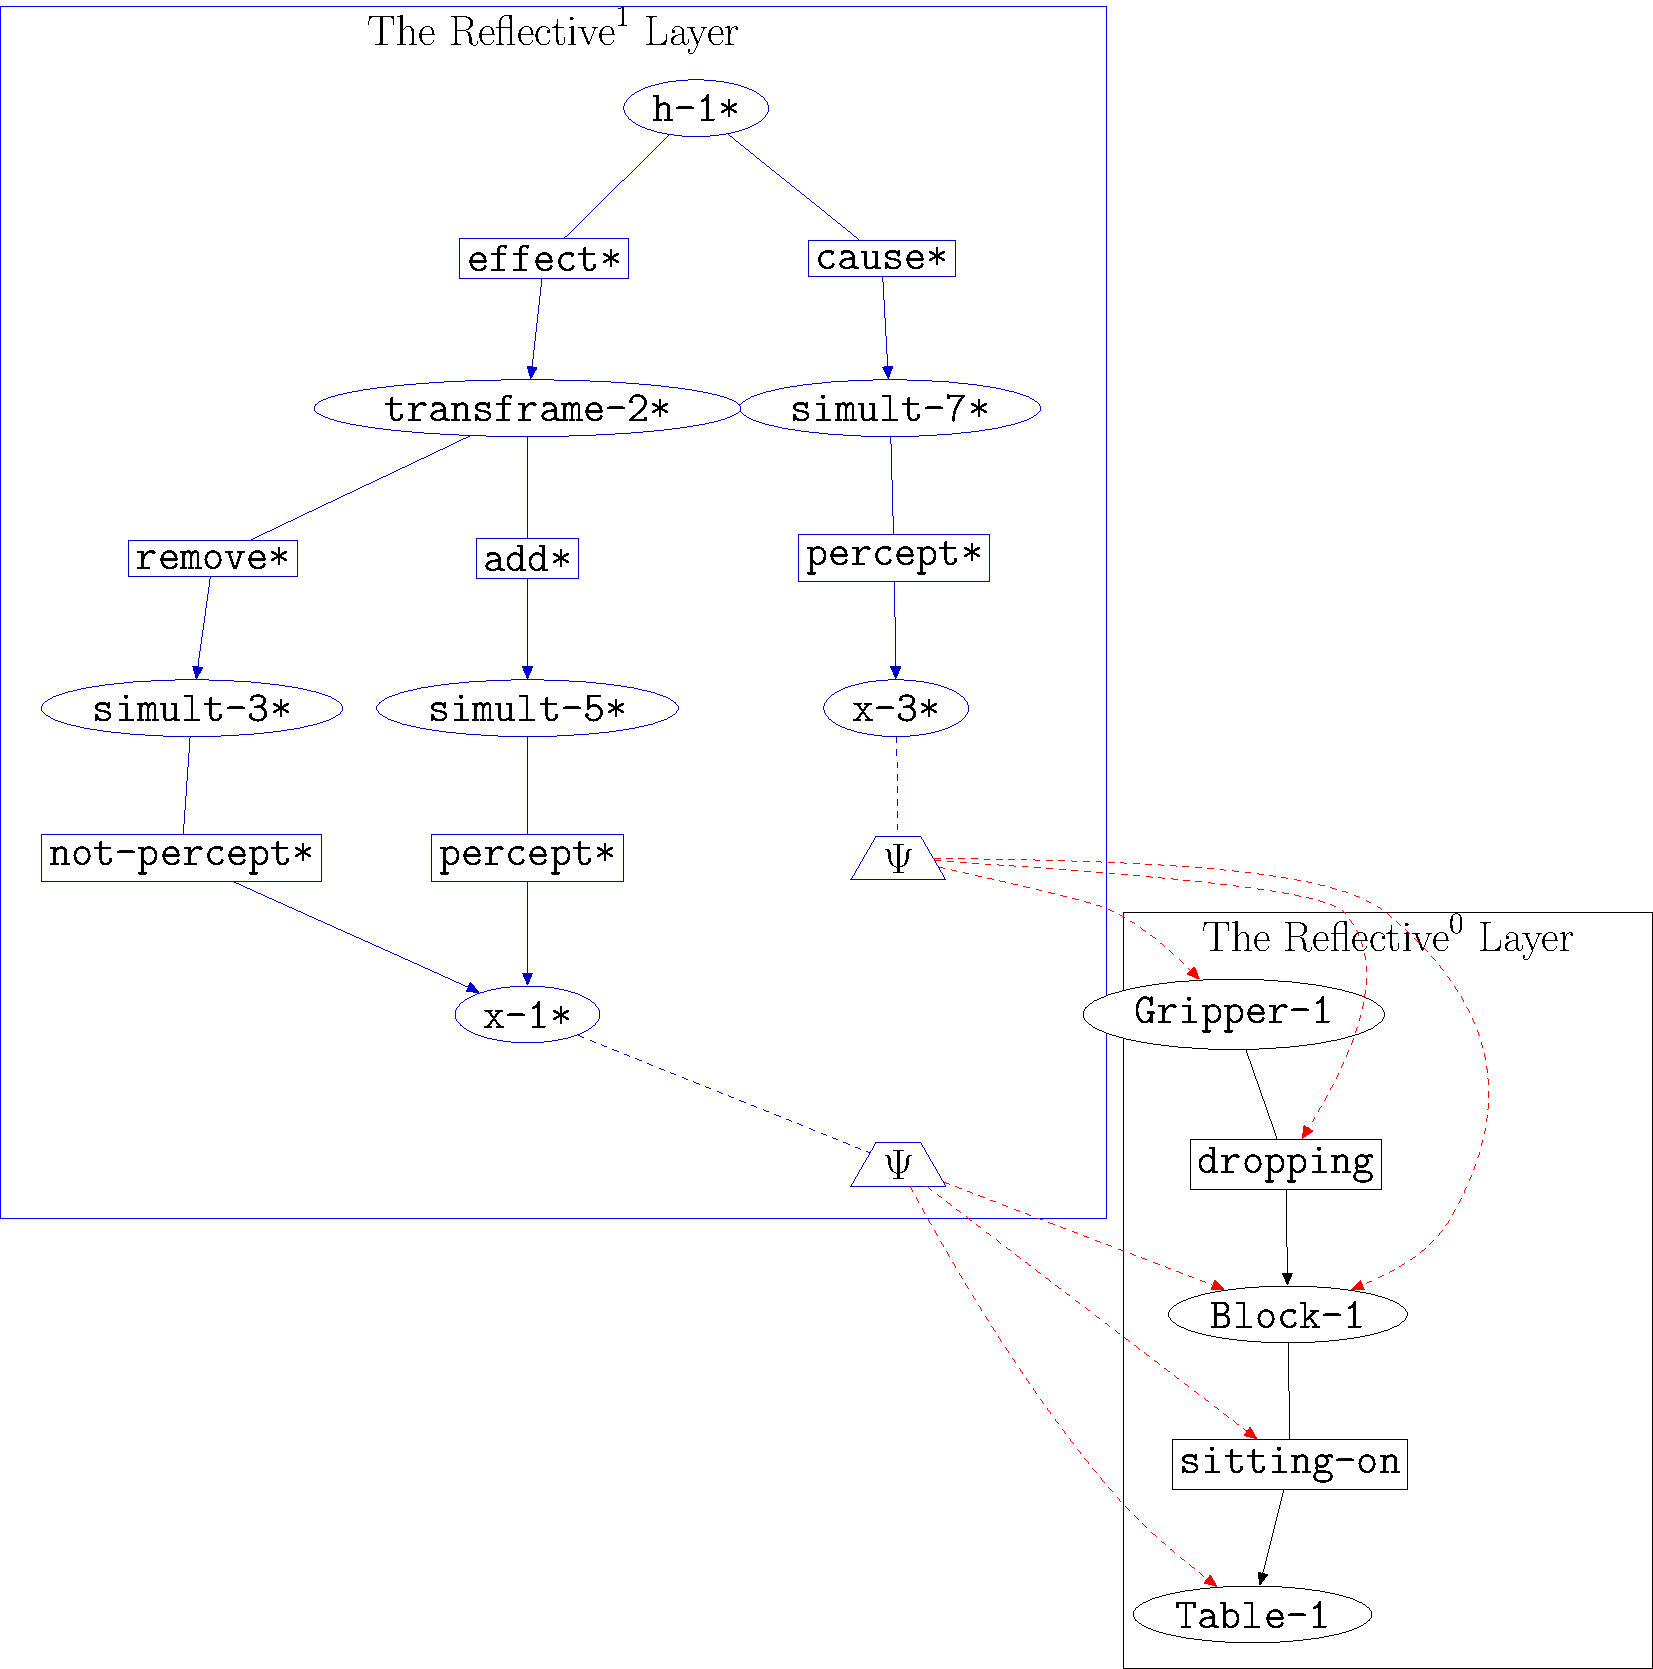
\includegraphics[width=12cm]{gfx/example_causal_hypothesis}
\caption[An example of a causal hypothesis.]{An example of a causal
  hypothesis, $h_1^*$, where the simultaneity,
  $\text{\tt{simult}}_7^*$, is hypothesized to be the cause of the
  transframe, $\text{\tt{transframe}}_2^*$.  In other words, the
  gripper dropping the block causes the block to be sitting on the
  table.}
\label{figure:example_causal_hypothesis}
\end{figure}

\section{Composing Plans from Hypotheses}

